% Deployment chapter continued
\section{Infrastructure from 5,000 feet}
Figure \ref{fig:infra5k} shows the final assembly of whirlpool crawler project. 
\begin{figure}[h!]
  \centering
  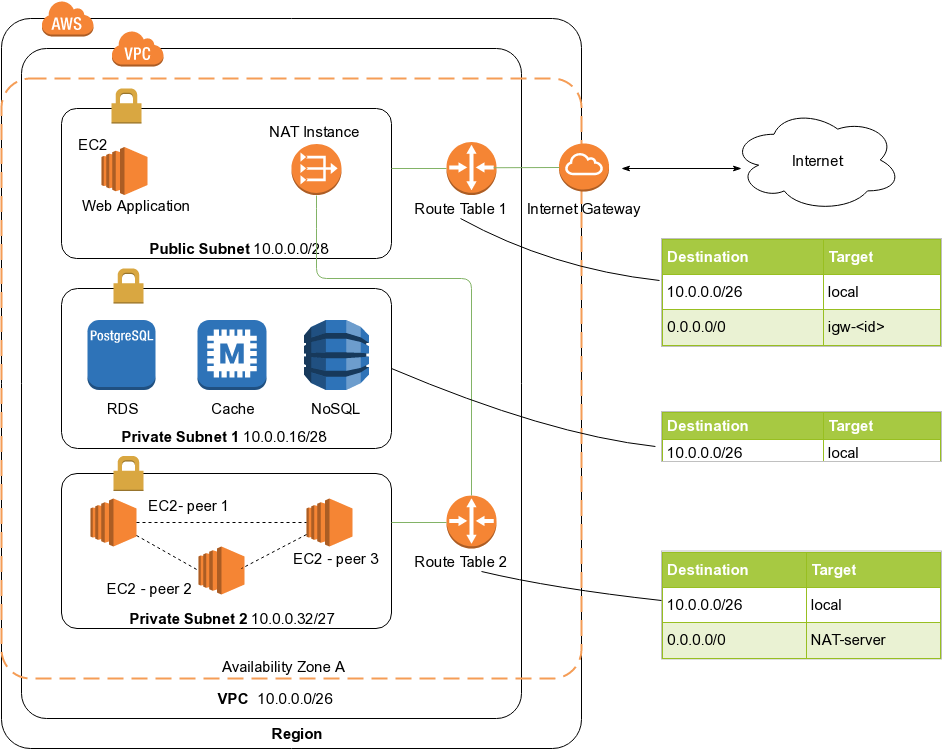
\includegraphics[width=20cm,height=12cm,keepaspectratio]{../media/crawler/aws-deploy-5k-feet.png}
  \caption{Whirlpool infrastructure with Route tables, NAT}
  \label{fig:infra5k}
\end{figure}

\noindent
Each subnet gets assigned a main route tables which cannot be deleted but instead can be overridden with custom route tables immediately effective on subnets as evident in figure \ref{fig:infra5k} with route tables 1 \& 2. Speaking of NAT instance in public subnet 1, is like any other AMI linux image but ships with pre-configured iptables. NAT forwards traffic from instances in subnet 4 to the internet and send the response for corresponding request back to those instances in subnet 4. It won't allow outside clients to initiate connections with instances in subnet 4. The custom route(shown in route table 2) directs the traffic originated within any of the private subnet peers matching subnet mask \ipAddress{0.0.0.0/0} to NAT server. The custom route(show in route table 1) scopes all packets matching \ipAddress{0.0.0.0/0} route to IGW. The traffic from private crawler subnet flows to NAT Instance and then to the IGW. The NAT translate back-and-forth source and destination IPs of private instances assuming external property - source/destination check is disabled.
\\
\\
\noindent
The subsystems of whirlpool leverage relational database(Amazon RDS) to maintain a history of URLs, NoSQL(EC2-mongoDB) to store extracted text. AWS does not have managed instance of MongoDB and requires the interested party to operate, maintain on an EC2 Instance. Also, later on, a cache server(AWS ElasticCache) can be adopted to optimize lookup efficiency against relational database by those subsystems dependent on it. Given this requirement, its safer to form a private subnet 2 dedicated to placement of data stores and in-memory cache as shown in the figure \ref{fig:infra5k}. This way, the data store subnet would stay safer accepting network connections within the VPC, specifically only from instances allowed by statefull firewalls(VPC security groups) attached to it. For relational database, amazon's RDS DB subnet group mandates 2 subnets, each in different availability zones to successfully launch the instance. Thus, a private subnet 3 in the figure.
\\
\\
Following are a list of VPC security groups in place for figure \ref{fig:infra5k} which regulate in/out
flow of traffic attached to EC2 instances, elasticCache, and RDS instance respectively.
\\
\begin{center}
  \begin{table}[h!]
  \begin{tabular}{| l | l | l | l | p{5cm} |}
    \textbf{Type} & \textbf{Protocol} & \textbf{Port Range} & \textbf{Source} & \textbf{Description} \\
    \hline
    SSH & TCP & 22 & sg-<bastion node> & only allows ssh to crawler nodes from bastion instance \\
    \hline
    Custom & TCP & 8080 & sg-<bastion node> & access RMQ management console access ssh tunneled to client host \\
  \end{tabular}
  \caption{Inbound rules of Security Group(sg) for EC2 crawler in private subnet 4}
  \end{table}
\end{center}

\begin{center}
  \begin{table}[h!]
    \begin{tabular}{| l | l | l | l | p{5cm} |}
      \textbf{Type} & \textbf{Protocol} & \textbf{Port Range} & \textbf{Source} & \textbf{Description} \\
      \hline
      SSH & TCP & 22 & sg-<bastion node> & ssh only from bastion instance \\
      \hline
      Custom & TCP & 27017 & sg-<crawler node> & mongo traffic from crawler nodes \\
      \hline
      Custom & TCP & 27017 & sg-<bastion node> & egress mongo traffic tunneled to client host \\
    \end{tabular}
    \caption{Inbound rules of Security Group(sg) for MongoDB in private subnet 2}
  \end{table}
\end{center}

\begin{center}
  \begin{table}[h!]
  \begin{tabular}{| l | l | l | l | p{5cm} |}
    \textbf{Type} & \textbf{Protocol} & \textbf{Port Range} & \textbf{Source} & \textbf{Description} \\
    \hline
    SSH & TCP & 22 & 0.0.0.0/0 & open to the world. Safely handle pvt. keys.\\
    \hline
    HTTP & TCP & 80 & sg-<crawler node> & accept non-ssl http traffic from crawler node \\
    \hline
    HTTPS & TCP & 443 & sg-<crawler node> & crawler downloads SSL HTTP traffic \\
  \end{tabular}
  \caption{Inbound rules of Security Group(sg) for bastion host in pub subnet 1}
  \end{table}
\end{center}

\pagebreak

\begin{center}
  \begin{table}[h!]
  \begin{tabular}{| l | l | l | l | p{5cm} |}
    \textbf{Type} & \textbf{Protocol} & \textbf{Port Range} & \textbf{Source} & \textbf{Description} \\
    \hline
    Custom & TCP & 5432 & sg-<crawler node> & accept sql request from crawler node \\
    \hline
    Custom & TCP & 5432 & sg-<bastion node> & egress rds tunneled to client host \\
  \end{tabular}
  \caption{Inbound rules of Security Group(sg) for AWS RDS in pvt subnet 2 and 3}
  \end{table}
\end{center}
\\
\begin{center}
  \begin{table}[h!]
  \begin{tabular}{| l | l | l | l | p{5cm} |}
    \textbf{Type} & \textbf{Protocol} & \textbf{Port Range} & \textbf{Source} & \textbf{Description} \\
    \hline
    Custom & TCP & 11211 & sg-<crawler node> & allow memcache traffic from crawler nodes \\
    \hline
    Custom & TCP & 11211 & sg-<bastion node> & egress cache traffic tunneled to client host \\
  \end{tabular}
  \caption{Inbound rules of Security Group(sg) for AWS ElastiCache in pvt subnet 2}
  \end{table}
\end{center}

\pagebreak

% Deployment chapter continued
\section{Bastion Host}
As per the wikipedia arcticle, a person named \emph{Marcus J. Ranum} defined the term \emph{bastion host} while discussing a article on firewalls as 
\begin{quote}
  "...a system identified by the firewall administrator as a critical strong point in the network security.
  Generally, bastion hosts will have some degree of extra attention paid to their security, may undergo
  regular audits, and may have modified software."
\end{quote}
Not necessarily in the context of AWS but also in data centers of IT organization, a baston host sole
purpose is to provide access to private network from external network such as internet. In a typical
AWS VPC setup, an instance in a public subnet with a security group that includes a inbound rule to
accept SSH traffic from trusted client host establishes secure remote connectivity after which the
instance(bastion host) acts a jumping point to ssh into various private instances belonging to various
private subnets within its VPC. With bastion host in place, a administrator uses ssh-agent
forwarding to authenticate to private instances. Agent forwarding doesn't require administrator to store
private keys on the bastion host and AWS best practices forbids storing private key files on servers.
Figure \ref{fig:infra5k} demonstrates a special network configuration where bastion host is placed in
DMZ zone separated from private, trusted networks such as subnets 2, 3, and 4. Another benefit bastion
hosts provide is not having to expose various management ports to internet to configure
utility/application services on private instances of the infrastructure.
\\
\\
\noindent
Agent forwarding is enabled by passing below flag when login into a remote node.

\begin{lstlisting}[language=bash]
  $ ssh -A user@ip
\end{lstlisting}
\\
\\
\noindent
Since whirlpool assembly contains multiple networks, following ssh aliases in .ssh/config saves from
typing.

%\begin{lstlisting}[language=Bash]
\begin{minted}[
  style=friendly,
  bgcolor=friendlybg,
  frame=lines,
  framesep=2mm,
  fontfamily=tt,
  baselinestretch=1.2,
  fontsize=\footnotesize,
  linenos
  ]{text}
# access to whirlpool bastion and its private nodes
Host whirlpool-bastion
   HostName ec2-x-x-x-x.us-east-2.compute.amazonaws.com
   User ec2-user
   IdentityFile ~/.ssh/whirlpool-jumbox.pem
   ProxyCommand none

Host whirlpool-crawler-1
   HostName ip-x-x-x-x.us-east-2.compute.internal
   User ubuntu
   IdentityFile ~/.ssh/whirlpool-jumbox.pem
   ProxyCommand ssh whirlpool-bastion -W %h:%p

Host whirlpool-mongodb
   HostName ip-x-x-x-x.us-east-2.compute.internal
   User ubuntu
   IdentityFile ~/.ssh/whirlpool-jumbox.pem
   ProxyCommand ssh whirlpool-bastion -W %h:%p
\end{minted}
%\end{lstlisting}

\pagebreak

\section{Monitoring services with SSH Tunnels}
This project steals concepts behind ssh tunnels \cite{tunnels} and applies them to its own AWS architecture, figure \ref{fig:infra5k}, to keep track of activities happening inside it. SSH tunnels are nicely explained by Scott Wiersdorf in his article; the source is listed in references. Image \ref{fig:simpletunnel} 
shows a \texttt{client-host} connecting to an example \texttt{web-server} on port 80 tunneled 
through \texttt{tunnel-host} using ssh utility.

\begin{figure}[h!]
  \centering
  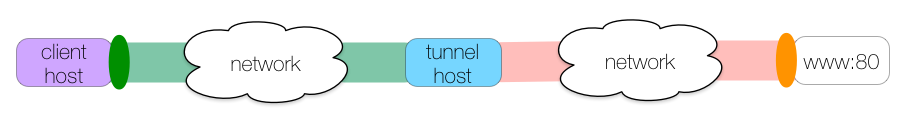
\includegraphics[width=15cm,height=5cm,keepaspectratio]{../media/crawler/simple-tunnel.png}
  \caption{simple tunnel \cite{tunnels}}
  \label{fig:simpletunnel}
\end{figure}

\noindent
SSH tunnels involves two hosts - \texttt{client-host}, and \texttt{tunnel-host}. The \texttt{client-host} specifies
the tunnel to be created. On the other hand, \texttt{tunnel-host} creates the tunnel connections. Both the hosts are defined as single bash command. The traffic between \texttt{client-host} to \texttt{tunnel-host} is secured by secure shell. All the  TCP traffic past the \texttt{tunnel-host} is not secured by SSH. The connections in SSH tunnels are initiated at only one end and so the listening end of the tunnel is referred to as tunnel \emph{ingress} and terminating end of the tunnel is referred to as tunnel \emph{egress} as 
illustrated in the image \ref{fig:poormanvpn}.

\begin{figure}[h!]
  \centering
  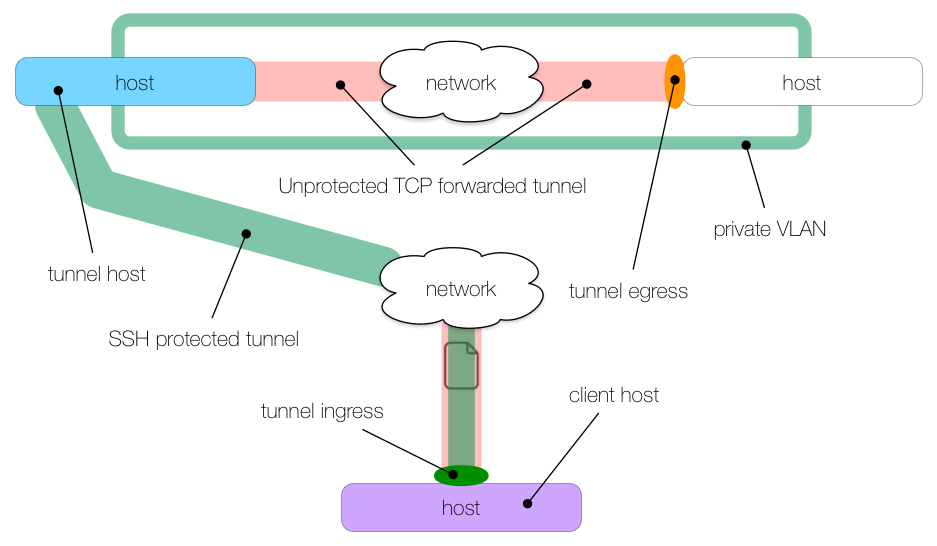
\includegraphics[width=15cm,height=12cm,keepaspectratio]{../media/crawler/ssh-tunnel-host-access.png}
  \caption{poor man's VPN \cite{tunnels}}
  \label{fig:poormanvpn}
\end{figure}

\pagebreak

\noindent
In the case of whirlpool network topology, \texttt{client-host} is the machine used to ssh into \texttt{bastion-host}. The \texttt{tunnel-host} is the \texttt{bastion-host}(NAT instance) and this is where the SSH connection ends. Bastion-host forwards TCP connection to a specified private instances within whirlpool AWS deployment because SSH agent-forwarding is enabled, discussed in previous section. The specified private instance is the egress and ingress is the \texttt{client-host} bound to a particular port.
\\
\\
\noindent
Following are the commands fired to monitor, diagnose services inside AWS. Note the egress 
\texttt{10.0.0.56:8080} and ingress is an omitted \texttt{localhost} on port \texttt{8080}.
The bastion host \texttt{whirlpool-bastion} forwards TCP to egress. \texttt{N} indicates no commands over SSH. This command is used for monitoring RabbitMQ server running on \texttt{10.0.0.56:8080}. The corresponding firewall rules is enabled for the same.

\begin{lstlisting}[language=bash]
  $ ssh -L 8080:10.0.0.56:8080 whirlpool-bastion -N
\end{lstlisting}
\\
\\
\noident
This command is used for making private ec2-mongodb instance available on \texttt{localhost}.
\begin{lstlisting}[language=bash]
  $ ssh -L 27017:10.0.0.26:27017 whirlpool-bastion -N
\end{lstlisting}
\\
\\
\noindent
This command is used for making private RDS instance available on \texttt{localhost}.
\begin{lstlisting}[language=bash]
  $ ssh -L 5432:whirlpool-postgres-prod.ytrewqgfdsa.us-east-2.rds.amazonaws.com:5432 whirlpool-bastion -N
\end{lstlisting}
\\
\\
\noindent
This command is used for making private memcache instance available on \texttt{localhost}.
\begin{lstlisting}[language=bash]
  $ ssh -L 11211:whirlpool-cache.qwerty.0001.use2.cache.amazonaws.com:11211 whirlpool-bastion -N
\end{lstlisting}

\pagebreak

\section{IAM and roles}\label{iamroles}
Showcase few IAM policies related to whirlpool project here.

\\
\\
\begin{figure}[h!]
  \centering
  
\includegraphics[width=14cm,height=14cm,keepaspectratio]{../media/crawler/iam_and_roles.png}
  \caption{Existing accounts and service role}
  \label{fig:iamroles}
\end{figure}

\noindent
This project is run under IAM whirlpool user with limited technical privileges by enforcing IAM policies, 
delegated by IAM administrator. The IAM administrator has full technical access but not billing access 
granted by AWS root user account. A service role exist because AWS cloudformation as a service provisions 
other services on behalf of whirlpool user by assuming a service role. Use of service role in context of 
this project is shown in figure \ref{fig:iamroles}.
\\
\\
\noindent
A service role contains a trust policy and permissions policy. Existing iam policies are added as 
permissions policy under 'actions'. Under 'resource/principal' property, cloudformation which assumes role is specified as a trust policy. A restricted IAM whirlpooluser doesn't need to be given permissions to create/modify/delete roles instead only list/describe/use roles. Note, this works only if IAM policies attached to
whirlpool IAM account has \texttt{IAM:passrole} action included.

\pagebreak

\noindent
Following are the restrictive, custom, managed IAM policies effective under whirlpool IAM account.

\begin{minted}[
  style=friendly,
  bgcolor=friendlybg,
  frame=lines,
  framesep=2mm,
  fontfamily=tt,
  baselinestretch=1.2,
  fontsize=\footnotesize,
  linenos
  ]{text}
whirlpool-user-iam-cache-vpc-policy.json
whirlpool-user-iam-cloudformation-policy.json
whirlpool-user-iam-cloudformation-role.json     
whirlpool-user-iam-cloudformation-s3-policy.json
whirlpool-user-iam-ec2-vpc-policy.json          
whirlpool-user-iam-policy.json
whirlpool-user-iam-rds-vpc-policy.json
\end{minted}

\noindent
Below is the code snippet of \texttt{whirlpool-user-iam-ec2-vpc-policy.json}, one of existing IAM policies
attached to IAM whirlpool account.
\inputminted[
fontfamily=tt,
baselinestretch=1.2,
fontsize=\footnotesize,
linenos,
numbersep=5pt,
tabsize=2,
frame=single]{js}{../../whirlpool/iam-policies/whirlpool-user-iam-ec2-vpc-policy.json}

\pagebreak